\section{Components}

This section aims to give a short review of the main techniques and architectures used in this thesis.

\subsection{LSTM}

\begin{figure}[p]
\centering
\includegraphics[width=0.9\linewidth]{rnn}
\caption{Architecture of a vanilla recurrent neural network cell. Each timestep some output and a hidden state vector \(\mathbf{h}_t\) are produced by looking at the hidden state vector from the previous timestep \(\mathbf{h}_{t-1}\) and the current input \(\mathbf{x}_t\). In this simple example, \(\mathbf{h}_t\) is also the output.}
\label{rnn}
\end{figure}

A recurrent neural network (RNN)\cite{rnn} is a special form of neural network that is used for sequential tasks. It works by having multiple copies of the network, one for each timestep. As the input proceeds in time, each network passes information to it's next instance as seen in figure \ref{rnn}. For an input sequence \((\mathbf{x}_1, ..., \mathbf{x}_n)\) the RNN produces at each timestep \(t\) a hidden state vector \(\mathbf{h}_t\) as follows:

\begin{equation*}
  \mathbf{h}_t = \tanh \left(\mathbf{W} \begin{pmatrix} \mathbf{x}_t \\ \mathbf{h}_{t-1} \end{pmatrix} \right)
\end{equation*}

\begin{figure}[p]
\centering
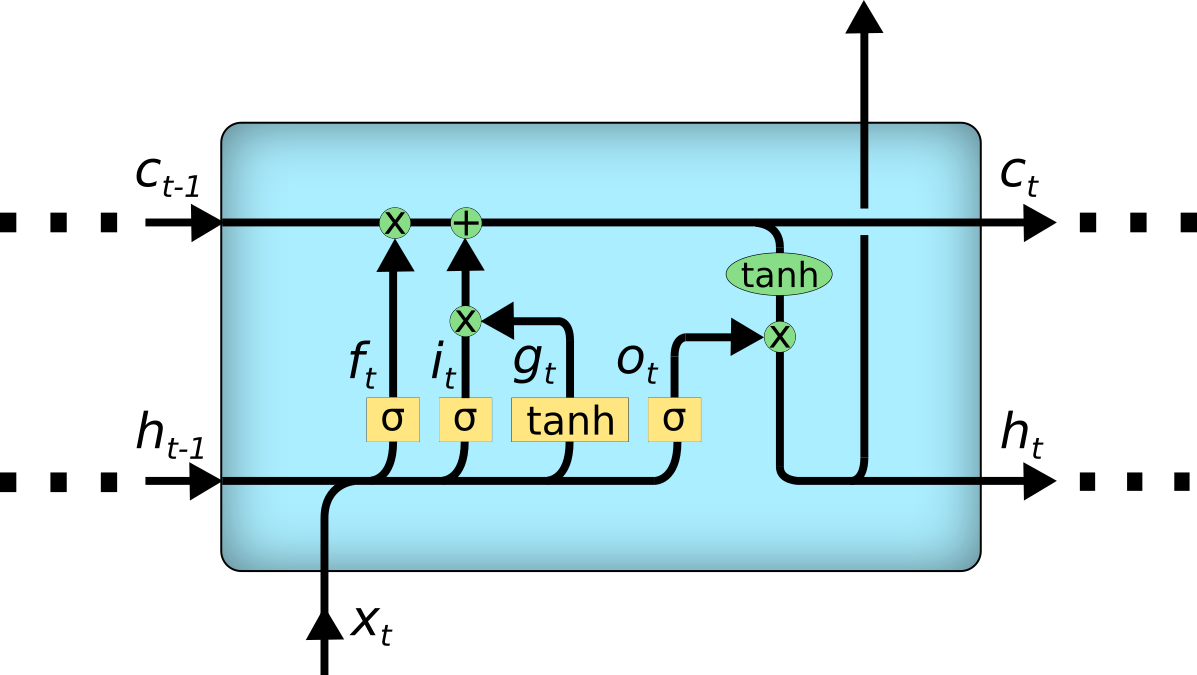
\includegraphics[width=0.9\linewidth]{lstm}
\caption{Architecture of a typical LSTM cell. In addition to the hidden state vector \(\mathbf{h}_t\), a memory state vector \(\mathbf{c}_t\) is passed to the next timestep. \(\mathbf{h}_{t-1}\) and the input \(\mathbf{x}_t\) are used to compute the gates \(\mathbf{f}_t\), \(\mathbf{i}_t\), \(\mathbf{g}_t\) and \(\mathbf{o}_t\). These gates are then used to add, delete and retrieve information to respectively from \(\mathbf{c}_{t-1}\), subsequently generating \(\mathbf{c}_t\) and \(\mathbf{h}_t\).}
\label{lstm}
\end{figure}

However, RNNs have proven to be hard to train, especially on long-range dependencies \cite{hochreiter_rnn}. In theory, they should be able to deal with these dependencies but either vanishing or exploding gradients usually prevent them from doing so. To solve this issue, Long Short-Term Memory networks (LSTMs) \cite{lstm} were proposed. In addition to \(\mathbf{h}_t\), LSTMs also pass a memory state vector \(\mathbf{c}_t\) to the next instance as can be seen in figure \ref{lstm}. The LSTM can choose at each timestep if it wants to read or forget information from the memory vector or write new information onto the vector. This is done by using explicit gating mechanisms:

\begin{align*}
  \mathbf{f}_t &= \sigma \left(\mathbf{W}_f \begin{pmatrix} \mathbf{x}_t \\ \mathbf{h}_{t-1} \end{pmatrix} \right) &
  \mathbf{i}_t &= \sigma \left(\mathbf{W}_i \begin{pmatrix} \mathbf{x}_t \\ \mathbf{h}_{t-1} \end{pmatrix} \right) \\
  \mathbf{o}_t &= \sigma \left(\mathbf{W}_o \begin{pmatrix} \mathbf{x}_t \\ \mathbf{h}_{t-1} \end{pmatrix} \right) &
  \mathbf{g}_t &= \tanh \left(\mathbf{W}_g \begin{pmatrix} \mathbf{x}_t \\ \mathbf{h}_{t-1} \end{pmatrix} \right)
\end{align*}

\noindent where \(\sigma\) is the sigmoid function. \(\mathbf{f}_t\), \(\mathbf{i}_t\) and \(\mathbf{o}_t\) can be thought of as binary gates that decide which information from \(\mathbf{c}_{t-1}\) should be deleted, which information of \(\mathbf{c}_{t-1}\) should be updated and which information from \(\mathbf{c}_t\) should be written to \(\mathbf{h}_t\).  Finally \(\mathbf{g}_t\) is a vector of possible values that (gated by \(\mathbf{i}_t\)) can be added to \(\mathbf{c}_{t-1}\) and because of the \(\tanh\) in the equation its values may range from \texttt{-1} to \texttt{1}. The state vectors are then updated as follows:

\begin{align*}
  \mathbf{c}_t &= \mathbf{f}_t \odot \mathbf{c}_{t-1} + \mathbf{i}_t \odot \mathbf{g}_t \\
  \mathbf{h}_t &= \mathbf{o}_t \odot \tanh(\mathbf{c}_t)
\end{align*}

Almost all state-of-the-art results today are achieved using either LSTMs or networks with a similar architecture like Gated Recurrent Units (GRUs) \cite{gru} because they are easier to train and excel at capturing long range dependencies.

\subsection{The Sequence-to-Sequence Model}

\begin{figure}[t]
\centering
\includegraphics[width=0.9\linewidth]{seq2seq}
\caption{The Sequence-to-Sequence Model applied to a translation example. The English source sentence is fed to the model word by word. After the input of an end-of-sequence token (\texttt{<eos>}), the network starts producing the output sentence in French. For this the produced output tokens are fed back to the network at the next timestep. The network signals the end of the sequence by outputting another \texttt{<eos>} token.}
\label{seq2seq}
\end{figure}

Traditional Deep Neural Networks (DNNs) process the whole input and then calculate some output, e.g. process an image and then classify it. This works well for problems where the input and the output are of a fixed dimension, however it is not suitable for problems where the input and the output are sequences of variable length. An example would be the input of a question and the network should produce an answer. We have seen that we can use LSTMs to process input sequences of variable length. However, in this case we want to process the whole input sequence and all the information that comes with it and only then start generating an output sequence. These problems are called sequence to sequence problems.

In \cite{seq2seq} the Sequence-to-Sequence Model is introduced as a solution to these problems. The model was applied to the task of Neural Machine Translation (NMT) and has since become the state of the art architecture in this field. The main concept can be seen in figure \ref{seq2seq}. First the whole input sequence is fed into the network and the output is ignored. Then we input an end-of-sequence token \texttt{<eos>} which signals the network to start producing the output. From there on the produced output tokens are fed to the network until the an end-of-sequence token is generated, thus signaling the end of the sequence. To speed up training the expected output is fed back to the network and not the actual produced output.

This architecture is further improved by splitting the network into two separate LSTMs. The first network takes all the input and encodes it into a vector which is then used to initialize the second network. It is first fed a start token \texttt{<GO>} and then the generated output until the end of the sequence is reached.

The network usually operates at word level and uses some word embedding like word2vec \cite{word2vec}. This method has the advantage of giving the input words some meaning through the embedding instead of just inputting a meaningless encoding of the word. While this is very effective for translation tasks, there are some limitations to this method. These embeddings work on a fixed size vocabulary which means that out of vocabulary words (OOV) can't be handled. Also special character sequences like \texttt{:)} pose a problem.

\subsection{Attention-Mechanism}

Attention is a relatively new concept for neural networks. The idea is to allow the network to chose on which information to focus at any given moment. For example in \cite{visual_attention} attention is used on the task of high resolution image classification. These kind of networks often struggle with memory constraints and attention can help them to only load the significant part of the image into the memory.

Attention has subsequently been applied to NMT \cite{attention_luong,attention_bahdanau}. The vector into which the input is encoded in the Sequence-to-Sequence model has been identified as a bottleneck which cuts down performance because of its limited capacity. After all the vector is of fixed dimensionality and needs to encode information about the whole input sequence. Because of that attention is used as a mean for the decoder to peek at previous hidden states of the encoder. This is done via a context vector \(\tilde{\mathbf{c}}_t\) which is combined with the current hidden state of the decoder \(\mathbf{h}_t\). The resulting attentional hidden state \(\tilde{\mathbf{h}}_t\) is then used by the decoder to generate the next output.

\begin{equation*}
  \tilde{\mathbf{h}}_t = \tanh \left(\mathbf{W}_c \begin{pmatrix} \tilde{\mathbf{c}}_t \\ \mathbf{h}_{t} \end{pmatrix} \right)
\end{equation*}

For the derivation of the context vector \(\tilde{\mathbf{c}}_t\) all hidden states of the encoder \(\bar{\mathbf{h}}_s\) are considered. For this an alignment vector \(\mathbf{a}_t\), whose size equals the input sequence length, is calculated from the current decoder hidden state \(\mathbf{h}_t\) and the encoder hidden states \(\bar{\mathbf{h}}_s\). The values of \(\mathbf{a}_t\) are then normalized using the softmax function.

\begin{equation*}
  a_{ts} = \frac
            {\exp(\score(\mathbf{h}_t, \bar{\mathbf{h}}_s))}
            {\sum_{s'} \exp(\score(\mathbf{h}_t, \bar{\mathbf{h}}_{s'}))}
\end{equation*}

Here, \(\score\) is a content-based function used to compare the decoder hidden state \(\mathbf{h}_t\) with each of the encoder hidden states \(\bar{\mathbf{h}}_s\). There are various possible choices for this function, for example:

\begin{equation*}
  \score(\mathbf{h}_t, \bar{\mathbf{h}}_s) =
  \begin{cases}
    \mathbf{h}_t^\intercal \mathbf{W}_a \bar{\mathbf{h}}_s \\
    \mathbf{v}_a^\intercal \tanh \left(\mathbf{W}_a \begin{pmatrix} \mathbf{h}_t \\ \bar{\mathbf{h}}_s \end{pmatrix} \right)
  \end{cases}
\end{equation*}

The context vector \(\tilde{\mathbf{c}}_t\) is then calculated as the weighted average over the encoder hidden states.

\begin{equation*}
  \tilde{\mathbf{c}}_t = \sum_{s'} a_{ts'} \bar{\mathbf{h}}_{s'}
\end{equation*}

\section{Model Implementation}

The implementation of the model used in this thesis is mostly based on the NMT model from Tensorflow \cite{seq2seq_tutorial}. The model consists of an encoder and a decoder with an implementation of the Luong attention mechanism \cite{attention_luong} wrapped around the latter one. The encoder and the decoder are both an LSTM cell consisting of 4 layers \`a 256 units each. No embedding was used because the model operates at the character level instead of the word level. This change was necessary because programming languages don't have a fixed vocabulary. The programmer is not restricted in the naming of variables, methods or the like and thus it makes no sense to restrict the model to a fixed vocabulary. This would only result in a lot of OOV tokens. Therefore the input is fed one character at a time to the model with the encoding of the character simply being its ASCII code, i.e. a number between 0 and 127.

For inference, the decoder was first fed a start-of-sequence token and after that the produced output was fed back as input to the decoder until an end-of-sequence token was output. During training however, the correct target sequence was fed to the decoder, left padded by a start-of-sequence token. This was done to optimize training because the token which would have been the correct output is fed to the decoder instead of the possibly wrong actual output.

 During backpropagation the gradients were clipped by a fixed norm. This technique is used to prevent the gradient from exploding \cite{gradient_clipping}. The norm chosen for this thesis is 5 but other values would also be possible (1 would be another common choice).

 The loss was measured with the cross-entropy loss function. Each timestep the decoder produces some output vector \(\mathbf{y}'^\intercal = \begin{pmatrix} y_1' & ... & y_n'\end{pmatrix}\). This vector is then normalized using the softmax function to get probabilities \(p_i\) for each possible output.

 \begin{equation*}
   p_i = \frac
             {\exp(y_i')}
             {\sum_{j} \exp(y_j')}
 \end{equation*}

 These probabilities are then used to compute the cross-entropy loss:

 \begin{equation*}
   l = - \sum_{j} y_j * \log(p_j)
 \end{equation*}

 Here \(\mathbf{y}^\intercal = \begin{pmatrix} y_1 & ... & y_n \end{pmatrix}\) is a one-hot target vector with \(y_i = 1\) for the desired output \(i\) and \(y_j = 0\) everywhere else.

 For each setting training was done for 30,000 iterations while the batch size was set to 64. The max sequence length was set to 300 meaning that only examples of 300 characters or less were used to train and evaluate the model.

\section{Dataset Construction}

To train the model, a big dataset of erroneous code examples produced by real programmers including their respective corrections would be ideal. This would assure a large variety of errors and real life examples. However such a dataset does not exist yet in part because the correction of erroneous code is a long and tedious work.

The best alternative is for the errors to be self introduced to a dataset of correct code. This task is no trivial one and several difficulties have to be taken into account and weighed up against each other. For one, the more sophisticated an error is the harder it is to introduce it consistently, but training a network on only easy errors (like missing semicolons) doesn't produce any added value. Another issue is the artificiality of the errors. One runs the risk of the model picking up on the error generation patterns and thus performing poorly on non-artificial examples. These problems are further discussed in subsection \ref{corruption}.

For this thesis, the data from the Java Github Corpus \cite{java_dataset} was chosen. As elaborated in section \ref{code_correction_section}, a weakly typed programming language like Python would be preferable over a strongly typed one like Java because a lot of errors in Java can already be found algorithmically. However, there is a general lack of large, diverse datasets of source code thus the selection of the Java Github Corpus. Furthermore, this thesis doesn't aim at building a fully polished "code corrector" but rather tries to test the boundaries of the possible. Also, the model knows nothing of the structure and rules of the programming language and therefore the capability of the model to grasp certain concepts can still be tested.

The dataset was crawled from Github and includes only projects which were forked at least once to assure a certain measure of quality. It consists of around 15,000 projects which amount to approximately 15GB of data.

\subsection{Preprocessing}

Before the data was used, some preprocessing had to be done. While LSTMs work better than vanilla RNNs on long range dependencies they still have their limits when it comes to input length \cite{timestep_limitation}. Because the input is fed to the network character-by-character rather than word-by-word, the input sequence can get quite long rather quickly. Thus the decision was made, to concentrate on method declarations because they are relatively self-contained and complex enough to introduce advanced errors while also being of manageable length.

The preprocessing was done for each Java file in the dataset separately and consisted of the following steps:

\begin{enumerate}
  \item All comments were removed from the file, because they are irrelevant for error detection and increase the sequence length.
  \item Line breaks were replaced by an end-of-line token.
  \item All unnecessary whitespaces were removed. This was also done to reduce sequence length because Java is a whitespace insensitive programming language, i.e. a Java program is still valid (albeit harder to understand) if its indentation is removed.
  \item If the file still contained non-ASCII characters, it was discarded. The purpose of this was to get rid of very rare characters, to reduce the input and output space and most importantly to avoid encoding errors.
  \item All method declarations were extracted from the file and checked on their corruptibility. This means, that all corruptions (see subsection \ref{corruption}) had to be able to be applied to the method. This assures that the defined corruption rate is met.
  \item All suitable methods were then written to new files (ca. 100MB each), one method per line.
\end{enumerate}

This resulted in around 1,7GB of train data.

\subsection{Corruptions}
\label{corruption}

As mentioned earlier, the generation of artificial errors is a challenging task. These errors need to be as sophisticated and as close to reality as possible else the learnt model cannot be applied to real world examples. Also a large variety in the introduced errors would be preferable. However these guidelines are not easy to implement especially for more sophisticated errors. While it is quite easy to introduce syntax errors such as a missing semicolon, the task of automatically and unfailingly generating logic errors is very challenging. That's why this thesis concentrates on five different errors of variable difficulty level.

The corruption of the data was done randomly during training. Each corruption was applied equally often, while the percentage of uncorrupted examples varied. Of the possible corruptions, two produced syntax errors, two semantic errors and one logic errors. The syntax errors consisted of removing a bracket or a semicolon, for the semantic errors a variable was misspelled or the return type of the method changed and the logic errors were produced by switching the order of two statement lines. Examples and implementation details of the different corruptions can be found in table \ref{corruption_table}.

Of the five possible corruptions, the syntax errors are the easiest to introduce and come relatively close to reality. They are typical errors that a novice programmer would produce and they are also the easiest to correct because the placement of semicolons and brackets follows strict rules. The other three corruptions produce more sophisticated errors but each one has some downsides.

The misspelling of a random variable works generally well. As a convention, the declaration of the variable is considered the "ground truth" and thus only occurrences of the variable after its declaration are misspelled. This is similar to how a traditional error checker would search for misspelled variables. However, there are some cases where the corruption doesn't work as intended. Consider the following code snippet:

\begin{lstlisting}[style=inline]
public int[] seedToArray(int seed){
  int[] seeds = new int[1];
  seeds[0] = seed;
  return seeds;
}
\end{lstlisting}

Lets assume that \texttt{seed} is to be corrupted. One possible misspelling would be to add a random character. If per chance an 's' is added to the end of the occurrence of \texttt{seed} in the third line, it produces another valid variable, namely \texttt{seeds}. Of course the error could still be detected but it is now a different type of error and the model shouldn't catch up on this unless it encounters such errors more frequently. It is also possible, that the corruption switches two adjacent characters in \texttt{seed}. If the second and third character are selected it would have no effect and therefore no error would be added. However these two scenarios are very specific and rare and therefore shouldn't impact the ability of the model to learn to find misspelled variables and correct them.

The other semantic error, the changing of the return type of the method, can be generated consistently but the generation imposes sometimes unsolvable problem to the network. One case is pretty simple. If the return type of the method is changed from \texttt{void} to something different, the model needs only check if a return statement is present and if not, the return type should be changed to \texttt{void}. The second case is more complicated as the return type is changed from one type to \texttt{void}. Again the model can determine if the return type \texttt{void} is correct by looking if a return statement is present. However if it determines that it is incorrect the model still needs to derive the correct return type from the given context which is not always possible. For example if the following source is given:

\begin{lstlisting}[style=inline]
public void incrementAndGetValue(){
  this.value += 1;
  return this.value;
}
\end{lstlisting}

\noindent the correct return type is not identifiable because \texttt{this.value} is not defined in the context of this method. It could be any numeric type. This is the tradeoff of only looking at methods opposed to whole files. However even with the full file context the return type could still be defined in another file, for example if the return type is determined by the return type of a method belonging to a different class. Despite this unsolvable problem the corruption can still be used to test the limits of what the model can learn.

Lastly logic errors are the most challenging ones to automatically generate because they require some form of understanding of the source code. To keep the errors relatively realistic, while also keeping the corruption as simple and as accurate as possible, the switching of the order of two adjacent lines in the method was chosen. However this corruption is not guaranteed to always produce a logic error. To further increase the probability of generating an error, some restrictions were put into place. Firstly, only variable declarations, assignments or method invocations were considered and secondly only two adjacent lines which were of a different type could be switched. This increased the probability of the occurrence of a logic error, but it still didn't guarantee it. Consider the following example:

\begin{lstlisting}[style=inline]
public int squareSum(int a, int b){
  int squareA;
  int squareB;
  squareA = a * a;
  squareB = b * b;
  return squareA + squareB;
}
\end{lstlisting}

Here the only lines that can be switched according to the restrictions listed above are line 3 and 4 but no logic error is produced in doing so. However to produce logic errors more consistently a deeper understanding of the code would be necessary which is not possible if the errors are to be generated artificially. Having said that, the corruption with its restrictions was still deemed "good enough" to do its purpose which was confirmed by the experiments.

\afterpage{
  \clearpage
  \pagestyle{empty}
  \begin{landscape}
    \begin{table}[t]
      \centering
      \begin{tabular}{ | m{4cm} m{2cm}  m{9cm}  m{5cm} | }
        \hline
        Corruption & Error Type & Explanation & Example \\
        \hline
        missing bracket &
        syntax &
        One random bracket (regular, curved or squared) is selected and removed from the source. &
        \lstinputlisting{listings/missing_bracket.java}
        \\
        missing semicolon &
        syntax &
        One random semicolon is selected and removed from the source. &
        \lstinputlisting{listings/missing_semicolon.java}
        \\
        misspelled variable &
        semantic &
        A random variable which is being declared in the source is selected. A random occurrence of the variable (except the one in the declaration) is then selected and misspelled. Possible misspellings are: removal of a random character, insertion of a random character, switch of two adjacent characters. &
        \lstinputlisting{listings/misspelled_variable.java}
        \\
        incorrect return type &
        semantic &
        The return type of the methods is changed. There are only two possibilities. If the return type is \texttt{void}, it is changed to one of Java's primitive data types (\texttt{int}, \texttt{float}, etc.). In any other case, the return type is changed to \texttt{void}. &
        \lstinputlisting{listings/incorrect_return_type.java}
        \\
        switched lines &
        logic &
        Two adjacent statement lines are switched in their order. As statement lines qualify variable declarations, assignments and method invocations. To increase the probability of an error, only lines of different types can be switched. &
        \lstinputlisting{listings/switched_lines.java}
        \\
        \hline
      \end{tabular}
      \caption{Implementation details and examples of all corruptions.}
      \label{corruption_table}
    \end{table}
  \end{landscape}
  \clearpage
}
